%% LyX 2.3.6 created this file.  For more info, see http://www.lyx.org/.
%DIF LATEXDIFF DIFFERENCE FILE
%DIF DEL manuscript_old.tex   Sat Aug 13 07:48:09 2022
%DIF ADD manuscript.tex       Wed Aug 24 15:12:57 2022
%% Do not edit unless you really know what you are doing.
\documentclass[review]{elsarticle}

\usepackage[unicode=true,colorlinks=false,hidelinks]{hyperref}
\usepackage[pagewise]{lineno}
\usepackage{float}
\usepackage{url}

%\modulolinenumbers[5]

\journal{Journal of Theoretical Biology}
\usepackage[T2A,LGR,T1]{fontenc}
%\usepackage{babel}
\usepackage{textcomp}
\usepackage{amstext}
\usepackage{amssymb}
\usepackage{stackrel}
\usepackage{graphicx}
\usepackage{subscript}
%\usepackage[unicode=true,pdfusetitle,
% bookmarks=true,bookmarksnumbered=false,bookmarksopen=false,
% breaklinks=false,pdfborder={0 0 0},pdfborderstyle={},backref=false,colorlinks=false]
% {hyperref}

%
\makeatletter
%%%%%%%%%%%%%%%%%%%%%%%%%%%%%% LyX specific LaTeX commands.



\DeclareRobustCommand{\greektext}{%
  \fontencoding{LGR}\selectfont\def\encodingdefault{LGR}}
\DeclareRobustCommand{\textgreek}[1]{\leavevmode{\greektext #1}}
\ProvideTextCommand{\~}{LGR}[1]{\char126#1}

\DeclareRobustCommand{\cyrtext}{%
  \fontencoding{T2A}\selectfont\def\encodingdefault{T2A}}
\DeclareRobustCommand{\textcyr}[1]{\leavevmode{\cyrtext #1}}

\newcommand{\lyxmathsym}[1]{\ifmmode\begingroup\def\b@ld{bold}
  \text{\ifx\math@version\b@ld\bfseries\fi#1}\endgroup\else#1\fi}


%%%%%%%%%%%%%%%%%%%%%%%%%%%%%% User specified LaTeX commands.
\makeatother

%\SectionNumbersOn
%\setkeys{acs}{doi = true}
\setkeys{Gin}{width=\linewidth}
\usepackage{subcaption}
\bibliographystyle{elsarticle-num}
%DIF PREAMBLE EXTENSION ADDED BY LATEXDIFF
%DIF UNDERLINE PREAMBLE %DIF PREAMBLE
\RequirePackage[normalem]{ulem} %DIF PREAMBLE
\RequirePackage{color}\definecolor{RED}{rgb}{1,0,0}\definecolor{BLUE}{rgb}{0,0,1} %DIF PREAMBLE
\providecommand{\DIFaddtex}[1]{{\protect\color{blue}\uwave{#1}}} %DIF PREAMBLE
\providecommand{\DIFdeltex}[1]{{\protect\color{red}\sout{#1}}}                      %DIF PREAMBLE
%DIF SAFE PREAMBLE %DIF PREAMBLE
\providecommand{\DIFaddbegin}{} %DIF PREAMBLE
\providecommand{\DIFaddend}{} %DIF PREAMBLE
\providecommand{\DIFdelbegin}{} %DIF PREAMBLE
\providecommand{\DIFdelend}{} %DIF PREAMBLE
\providecommand{\DIFmodbegin}{} %DIF PREAMBLE
\providecommand{\DIFmodend}{} %DIF PREAMBLE
%DIF FLOATSAFE PREAMBLE %DIF PREAMBLE
\providecommand{\DIFaddFL}[1]{\DIFadd{#1}} %DIF PREAMBLE
\providecommand{\DIFdelFL}[1]{\DIFdel{#1}} %DIF PREAMBLE
\providecommand{\DIFaddbeginFL}{} %DIF PREAMBLE
\providecommand{\DIFaddendFL}{} %DIF PREAMBLE
\providecommand{\DIFdelbeginFL}{} %DIF PREAMBLE
\providecommand{\DIFdelendFL}{} %DIF PREAMBLE
%DIF HYPERREF PREAMBLE %DIF PREAMBLE
\providecommand{\DIFadd}[1]{\texorpdfstring{\DIFaddtex{#1}}{#1}} %DIF PREAMBLE
\providecommand{\DIFdel}[1]{\texorpdfstring{\DIFdeltex{#1}}{}} %DIF PREAMBLE
\newcommand{\DIFscaledelfig}{0.5}
%DIF HIGHLIGHTGRAPHICS PREAMBLE %DIF PREAMBLE
\RequirePackage{settobox} %DIF PREAMBLE
\RequirePackage{letltxmacro} %DIF PREAMBLE
\newsavebox{\DIFdelgraphicsbox} %DIF PREAMBLE
\newlength{\DIFdelgraphicswidth} %DIF PREAMBLE
\newlength{\DIFdelgraphicsheight} %DIF PREAMBLE
% store original definition of \includegraphics %DIF PREAMBLE
\LetLtxMacro{\DIFOincludegraphics}{\includegraphics} %DIF PREAMBLE
\newcommand{\DIFaddincludegraphics}[2][]{{\color{blue}\fbox{\DIFOincludegraphics[#1]{#2}}}} %DIF PREAMBLE
\newcommand{\DIFdelincludegraphics}[2][]{% %DIF PREAMBLE
\sbox{\DIFdelgraphicsbox}{\DIFOincludegraphics[#1]{#2}}% %DIF PREAMBLE
\settoboxwidth{\DIFdelgraphicswidth}{\DIFdelgraphicsbox} %DIF PREAMBLE
\settoboxtotalheight{\DIFdelgraphicsheight}{\DIFdelgraphicsbox} %DIF PREAMBLE
\scalebox{\DIFscaledelfig}{% %DIF PREAMBLE
\parbox[b]{\DIFdelgraphicswidth}{\usebox{\DIFdelgraphicsbox}\\[-\baselineskip] \rule{\DIFdelgraphicswidth}{0em}}\llap{\resizebox{\DIFdelgraphicswidth}{\DIFdelgraphicsheight}{% %DIF PREAMBLE
\setlength{\unitlength}{\DIFdelgraphicswidth}% %DIF PREAMBLE
\begin{picture}(1,1)% %DIF PREAMBLE
\thicklines\linethickness{2pt} %DIF PREAMBLE
{\color[rgb]{1,0,0}\put(0,0){\framebox(1,1){}}}% %DIF PREAMBLE
{\color[rgb]{1,0,0}\put(0,0){\line( 1,1){1}}}% %DIF PREAMBLE
{\color[rgb]{1,0,0}\put(0,1){\line(1,-1){1}}}% %DIF PREAMBLE
\end{picture}% %DIF PREAMBLE
}\hspace*{3pt}}} %DIF PREAMBLE
} %DIF PREAMBLE
\LetLtxMacro{\DIFOaddbegin}{\DIFaddbegin} %DIF PREAMBLE
\LetLtxMacro{\DIFOaddend}{\DIFaddend} %DIF PREAMBLE
\LetLtxMacro{\DIFOdelbegin}{\DIFdelbegin} %DIF PREAMBLE
\LetLtxMacro{\DIFOdelend}{\DIFdelend} %DIF PREAMBLE
\DeclareRobustCommand{\DIFaddbegin}{\DIFOaddbegin \let\includegraphics\DIFaddincludegraphics} %DIF PREAMBLE
\DeclareRobustCommand{\DIFaddend}{\DIFOaddend \let\includegraphics\DIFOincludegraphics} %DIF PREAMBLE
\DeclareRobustCommand{\DIFdelbegin}{\DIFOdelbegin \let\includegraphics\DIFdelincludegraphics} %DIF PREAMBLE
\DeclareRobustCommand{\DIFdelend}{\DIFOaddend \let\includegraphics\DIFOincludegraphics} %DIF PREAMBLE
\LetLtxMacro{\DIFOaddbeginFL}{\DIFaddbeginFL} %DIF PREAMBLE
\LetLtxMacro{\DIFOaddendFL}{\DIFaddendFL} %DIF PREAMBLE
\LetLtxMacro{\DIFOdelbeginFL}{\DIFdelbeginFL} %DIF PREAMBLE
\LetLtxMacro{\DIFOdelendFL}{\DIFdelendFL} %DIF PREAMBLE
\DeclareRobustCommand{\DIFaddbeginFL}{\DIFOaddbeginFL \let\includegraphics\DIFaddincludegraphics} %DIF PREAMBLE
\DeclareRobustCommand{\DIFaddendFL}{\DIFOaddendFL \let\includegraphics\DIFOincludegraphics} %DIF PREAMBLE
\DeclareRobustCommand{\DIFdelbeginFL}{\DIFOdelbeginFL \let\includegraphics\DIFdelincludegraphics} %DIF PREAMBLE
\DeclareRobustCommand{\DIFdelendFL}{\DIFOaddendFL \let\includegraphics\DIFOincludegraphics} %DIF PREAMBLE
%DIF COLORLISTINGS PREAMBLE %DIF PREAMBLE
\RequirePackage{listings} %DIF PREAMBLE
\RequirePackage{color} %DIF PREAMBLE
\lstdefinelanguage{DIFcode}{ %DIF PREAMBLE
%DIF DIFCODE_UNDERLINE %DIF PREAMBLE
  moredelim=[il][\color{red}\sout]{\%DIF\ <\ }, %DIF PREAMBLE
  moredelim=[il][\color{blue}\uwave]{\%DIF\ >\ } %DIF PREAMBLE
} %DIF PREAMBLE
\lstdefinestyle{DIFverbatimstyle}{ %DIF PREAMBLE
	language=DIFcode, %DIF PREAMBLE
	basicstyle=\ttfamily, %DIF PREAMBLE
	columns=fullflexible, %DIF PREAMBLE
	keepspaces=true %DIF PREAMBLE
} %DIF PREAMBLE
\lstnewenvironment{DIFverbatim}{\lstset{style=DIFverbatimstyle}}{} %DIF PREAMBLE
\lstnewenvironment{DIFverbatim*}{\lstset{style=DIFverbatimstyle,showspaces=true}}{} %DIF PREAMBLE
%DIF END PREAMBLE EXTENSION ADDED BY LATEXDIFF

\begin{document}

\begin{frontmatter}

\title{Mechanisms of detachment in fibrillar adhesive systems}


\author[mymainaddress]{Pranav Sudersan}

\author[mymainaddress]{Michael Kappl\corref{mycorrespondingauthor}}
\cortext[mycorrespondingauthor]{Corresponding author. \emph{Telephone:} +49 6131 379-114}
\ead{kappl@mpip-mainz.mpg.de}

\address[mymainaddress]{Max Planck Institute for Polymer Research, Ackermannweg 10, 55128
Mainz, Germany}

\begin{abstract}
Several creatures can climb on smooth surfaces with the help of hairy
adhesive pads on their legs. A rapid change from strong attachment
to effortless detachment of the leg is enabled by the asymmetric geometry
of the tarsal hairs. In this study, we propose mechanisms by which
the hairy pad can be easily detached, even when the hairs possess no
asymmetry. Here, we examine the possible function of the tibia-tarsus leg joint and the claws. Based on a spring-based model, we consider three modes
of detachment: vertically pulling the pad while maintaining either
a 1) fixed or a 2) free joint, or by 3) flexing the pad about
the claw. We show that in all cases, the adhesion force can be significantly
reduced due to elastic forces when the hairs deform non-uniformly
across the array. %, an effect that we call ``\emph{elastic weakening}''.
Our proposed model illustrates the design advantage of such fibrillar
adhesive systems, that not only provide strong adhesion, but also
allow easy detachment, making them suitable as organs for fast locomotion and reliable hold.
The presented approaches can be potentially used to switch the adhesion
state in bio-inspired fibrillar adhesives, by incorporating artificial joints and claws into their design, without the need of asymmetric or stimuli-responsive fibrillar structures.
\end{abstract}

\begin{keyword}
fibrillar adhesion \sep reversible adhesion \sep contact splitting \sep beetle \sep biomechanics 
\end{keyword}

\end{frontmatter}

\linenumbers

\section{Introduction}

Over the past few decades, there have been numerous studies to understand
how animals, such as geckos and insects, are able to walk on surfaces
of any direction while seemingly defying gravity. A microscopic observation
reveals that, in many cases, animals have a dense array of fibrillar structures
at the end of their legs \cite{RN198,RN59}. These \emph{hairy} adhesive
pads help the animal to stay attached to any surface or detach easily
at will for countless cycles, a property that is referred to as \emph{reversible
adhesion}. Previous attempts to theoretically explain adhesion in
hairy pads \cite{RN40,RN120,Popov2016BiologicalMW} has followed two fundamental approaches: either by energy balance, or by force balance. 

In the energy balance approach, adhesion is usually characterized by \emph{work
of adhesion} (W\textsubscript{adh}), which is the energy required
to separate a pad from the surface. During detachment, the elastic
energy stored in the hair is dissipated, that increases W\textsubscript{adh}
and thus adhesion is enhanced \cite{RN29,RN114}. Detachment of an
individual hair can be explained based on Kendall's peeling theory \cite{RN147, RN296},
which predicts low adhesion at high peeling angles.

In the force balance approach, adhesion is characterized by \emph{pull-off
force}, F\textsubscript{p} (or stress, \textgreek{sv}\textsubscript{p}),
which is the minimum force necessary to separate two surfaces from
contact. Based on a \emph{cohesive zone model}, Hui et. al. \cite{RN72}
have identified two regimes of single hair detachment: 1) a \emph{flaw sensitive}
regime, where, for large hair radius, contact failure occurs due to crack propagation, 
initiated by a stress singularity at the edge of the hair, leading
to low \textgreek{sv}\textsubscript{p}; 2) a \emph{flaw insensitive} regime,
where, for small hair radius, the contact interface fails simultaneously, leading to high
\textgreek{sv}\textsubscript{p}. Likewise, Tian et. al. \cite{RN230} have shown
that the spatula-shaped hair tips in a gecko's toe allows it
to change adhesion by three orders of magnitude by laterally sliding
and controlling the pulling angle to disorient the hairs. The detailed mechanics of the
spatula-shaped hair design for controlling adhesion have been extensively studied by theoretical modelling \cite{pantano2011, sauer2013, Wu2015, kligerman2020, Grill2021, Gouravaraju2021}, artificial mimics \cite{RN57, Murphy2007, Menguc2012, Chary2013, Kim2017} as well as in several biological systems \cite{autumn2000,Langer2004,Varenberg2010}. Federle \cite{RN20}
has further argued that the curved shape of the hair helps the pad
to stay attached when pulled proximally and easily detached by elastic
recoil when pushed distally. 

The theory presented so far suggests that a low detachment force of
a fibrillar adhesive pad can be achieved either by increasing the stress concentration
by peeling the pad at high angles, or by laterally shearing the pad
before pull-off, which requires the hairs to have an asymmetric geometry
or curvature. However, some insects like male dock beetles predominantly
possess mushroom-shaped hairs with flat discoid terminals on their pads \cite{RN19},
that are relatively less asymmetric compared to the spatula-shaped hairs. These mushroom-shaped hairs have in fact been shown to possess superior
adhesion compared to the spatula-shaped hairs \cite{RN112,RN57} and are generally resistant to detachment via lateral shear \cite{Heepe2014}. Yet, how does the beetles possessing such mushroom-shaped hairs still easily detach their legs during locomotion? Besides, from an application perspective, introducing asymmetry
into the pillar geometry to construct spatula-shaped artificial biomimetic 
adhesives for easy detachment is challenging due to current limitations in fabrication techniques and difficulty in scaling-up \cite{RN57}.
Alternate strategies are thus desired to switch the adhesion state
of symmetric pillar arrays in a reversible manner. This can be achieved, for example, by buckling
the pillars under compressive load leading to their contact loss \cite{RN279}
or by using special materials reacting to external stimuli such as
magnetic field \cite{RN186}, UV light \cite{RN280} or temperature \cite{RN281}.

Employing the force-balance approach, in this work we theoretically model the possible mechanisms by which adhesive pads with axially-symmetric hairs can be easily detached, without the need of any spatula-like asymmetry. 
Here, we focus our analysis on normal adhesion force necessary to separate 
the pad from a flat surface under a purely mechanical action. We found that the maximum force necessary to detach the leg can be significantly reduced by strategically controlling the tilt, joints and claws of the adhesive system. We hope our work to provide new approaches to control the adhesion force
of an artificial micro-pillar adhesive, that has applications in
bio-inspired climbing robots, pick-and-place operations and reusable
adhesives.

\section{Model}

Similar to previous approaches \cite{RN117, RN253}, the fibrillar adhesive pad is assumed to be a one-dimensional array of $N_{t}$
hairs, each behaving like a spring with spring constant, $k_{h}$,
and natural length, $l_{h,0}$ (Figure \ref{fig:Schematic}). The
array backing is assumed to be stiff. The pad is attached to a linearly
deformable leg (tibia), assumed to be another spring with spring constant,
$k_{l}$, and natural length, $l_{l,0}$. The leg is hinged to the
array at a distance, $s$, from the right end of the array. The hinge, analogous to the tibia-tarsus leg joint of an insect, 
is at a vertical distance, $d_{s}$, from the surface. The hairs are
spaced apart by a width, $w$, and the array is of length, $L=\left(N_{t}-1\right)w$.
The pad is oriented at an instantaneous angle, $\theta$, while making contact with
a flat smooth surface. Each hair can attain a maximum length, $l_{h,p}$,
before pull-off, such that its pull-off force, $f_{p}=k_{h}\left(l_{h,p}-l_{h,0}\right)$.
$F_{net}$ is the net normal force on the pad and $M_{net}$ is the the net
moment about the hinge, at a particular instant during the detachment
process. We focus only on vertical detachment modes and thus lateral friction forces between the hairs and surface are not considered for our analysis.

\begin{figure}[H]
\includegraphics{Figure1-model_schematic}\caption{\textbf{Spring contact model of a fibrillar adhesive pad.} The pad consists of
an array of $N_{t}$ hairs connected to a deformable leg at the joint.
At a particular distance, $d_{s}$, $n$ number of hairs are in contact
and the array is oriented at a tilt angle, $\theta$, with the surface.
\label{fig:Schematic}}
\end{figure}

Suppose at a particular instant, there are $n$ hairs in contact with
the surface. The net force on the whole pad will be,

\[
F_{net}=\stackrel[i=1]{n}{\sum}k_{h}\left(l_{h,i}-l_{h,0}\right)
\]

Simplifying, we get (see Appendix \DIFdelbegin \DIFdel{A }\DIFdelend \DIFaddbegin \DIFadd{B }\DIFaddend for derivation):

\begin{equation}
F_{net}=nk_{h}\left[d_{s}-l_{h,0}-\Psi\sin\theta\right]\label{eq:force_n_d}
\end{equation}

where, $\Psi=s-\frac{n-1}{2}w$. For a particular value of $n$, equation
(\ref{eq:force_n_d}) is valid until a certain distance, $d_{s,max}$,
above which the left most hair will detach. Just before detachment,
this hair will be at its maximum length, $l_{h,p}$. From simple geometry
we can thus find:

\begin{equation}
d_{s,max}=l_{h,0}+\frac{f_{p}}{k_{h}}+\left[s-\left(n-1\right)w\right]\sin\theta\label{eq:d_max}
\end{equation}

Equation (\ref{eq:force_n_d}) will be valid for $d_{s}\leq d_{s,max}$.

The maximum possible adhesion of the array would be the case when
all hairs detach simultaneously ($\theta=0\lyxmathsym{\textdegree}$):

\begin{equation}
F_{max}=N_{t}f_{p}\label{eq:simul_detach}
\end{equation}

The net moment, $M_{net}$, about the joint can be similarly derived
(see Appendix \DIFdelbegin \DIFdel{A}\DIFdelend \DIFaddbegin \DIFadd{B}\DIFaddend ):

\begin{equation}
M_{net}=nk_{h}\cos\theta\left[\left(d_{s}-l_{h,0}\right)\Psi-\left\{ \Psi^{2}+\frac{n^{2}-1}{12}w^{2}\right\} \sin\theta\right]\label{eq:moment_n_d}
\end{equation}

Let us now consider the scenario where even the leg above the joint
can undergo elastic stretching together with the hairs. When a hair
detaches from the surface, the leg undergoes an elastic recoil due
to the stored elastic energy. Suppose the leg relaxes upward by a
recoil length, $\Delta l$. For $n$ hairs in contact, the force balance
before and after a hair detaches is given respectively by:

\[
\begin{array}{c}
\stackrel[i=1]{n}{\sum}k_{h}\left(l_{h,i}-l_{h,0}\right)=k_{l}\left(l_{l}-l_{l,0}\right)\\
\stackrel[i=1]{n-1}{\sum}k_{h}\left(l_{h,i}+\Delta l-l_{h,0}\right)=k_{l}\left(l_{l}-\Delta l-l_{l,0}\right)
\end{array}
\]

Solving the above two equations for $\Delta l$, we get:

\begin{equation}
\Delta l=\frac{f_{p}}{k_{h}\left(n-1\right)+k_{l}}\label{eq:backing_deform}
\end{equation}

Thus, $d_{s}$ shifts by $\Delta l$ in equations \ref{eq:force_n_d}
and \ref{eq:moment_n_d} at each event of hair detachment (i.e. when
$d_{s}=d_{s,max}$).

We express the forces and distances in non-dimensional forms, as below:

\[
\hat{f}_{p}=\frac{f_{p}}{k_{h}w},\quad\hat{F}_{net}=\frac{F_{net}}{k_{h}w},\quad\hat{d_{s}}=\frac{d_{s}-l_{h,0}}{w},\quad\hat{s}=\DIFdelbegin \DIFdel{\frac{s}{w}
}\DIFdelend \DIFaddbegin \DIFadd{\frac{s}{L}
}\DIFaddend \]

Here, $\hat{f_{p}}$ is a parameter which encapsulates the hair's
adhesion force, stiffness and array density. Unless specified, positive
force values represent attraction by convention.

\section{Detachment mechanisms}

We consider three tentative scenarios to detach the adhesive pad from
a surface: 1) \emph{Fixed pull}, where the pad is pulled vertically
up while keeping a fixed joint; 2) \emph{Free pull,} where the
pad is pulled vertically up while keeping the joint free to allow
rotation of the array; 3) \emph{Flex}, where the pad is hinged
to an external point (claw-hinge), and detached in a rotary fashion,
emulating the claw function in insects. To investigate each case in
detail, let us assume a pad to be a one-dimensional analogue of a 
dock beetle's adhesive pad \cite{RN19, RN79} with $N_{t}=25$ hairs and $\hat{f_{p}}=0.1$
(see discussion on \emph{detachment pathways} for details) attached to a stiff leg (or tibia) with $k_{l}\rightarrow\infty$. The situation
of a soft leg with $k_{l}/k_{h}=10$ is also considered for the first
two cases involving vertical detachment.

\subsection{Fixed pull}

\begin{figure}[H]
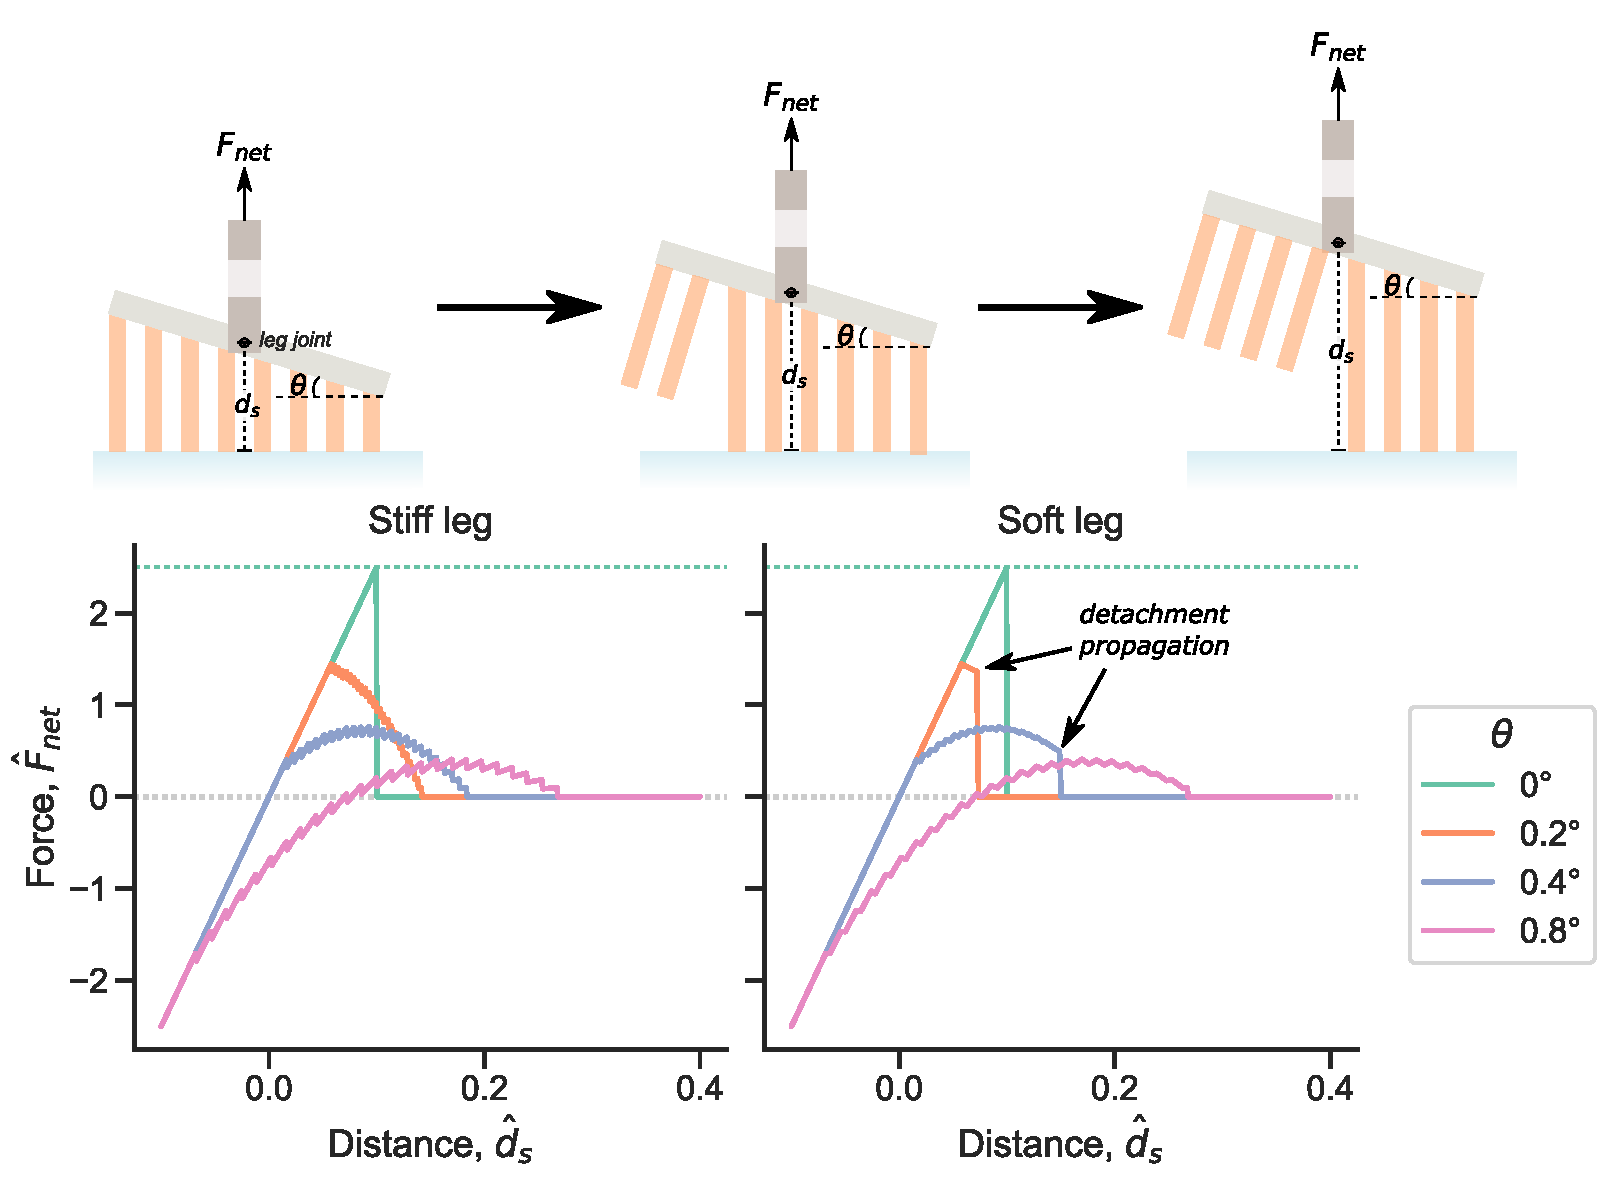
\includegraphics{Case1-Fixed_pull}\caption{\textbf{Detachment by \emph{Fixed Pull}.} 
Force-distance curves for a fibrillar adhesive pad, pulled vertically upwards with
a fixed joint. The
tilt angle, $\theta$, of the array is kept fixed during detachment.
The leg (tibia) is either stiff ($k_{l}\rightarrow\infty$) or soft ($k_{l}/k_{h}=10$).
Positive force values represent attraction between the array and the surface. The green dashed line
represents the maximum possible adhesion for the pad. All values are
normalized to dimensionless forms, as described in text.\label{fig:Fixed-pull}}
\end{figure}

The fibrillar adhesive pad can be detached by pulling it vertically upwards
while maintaining a constant tilt angle, $\theta$, with the surface.
This can be achieved if the joint is kept fixed. 
Equations \ref{eq:force_n_d}, \ref{eq:d_max}
and \ref{eq:simul_detach} can be used to get the resulting force-distance
curves for such a scenario. 

Increasing the tilt of the pad decreases its maximum force or adhesion
(Figure \ref{fig:Fixed-pull}). Tilting the pad causes an inhomogeneous
deformation of hairs, where, on one end they are stretched, while,
on the other end they are compressed. The balance of the respective
attractive and repulsive elastic forces of the hairs ultimately results
in a decrease in the net force. The tilted orientation also causes
the individual hairs to detach distinctly rather than simultaneously,
further reducing the maximum adhesion of the array. We term this
effect of loss in adhesion due to a non-uniform hair deformation across
the array as \emph{elastic weakening}. When there is no tilt
($\theta=0\lyxmathsym{\textdegree}$), all the hairs undergo identical
deformation and ultimately detach simultaneously after a distance,
$\hat{d_{s}}=0.1$. Here, no \emph{elastic weakening} occurs and the
pad shows the maximum possible adhesion.

For the case of a stiff leg (tibia), we see that at small distances, all hairs
of the pad are in contact with the surface, resulting in a linear
force response. On further pulling, the hairs will start to detach
sequentially from left to right, indicated by a characteristic saw-tooth
jitter in the force curves. The hairs of the pad with a higher tilt
angle will start to detach first, followed by the ones with a lower
tilt. 

For the case of a soft leg (tibia), we observe a similar effect of tilt angle
on the force curves as before. The maximum adhesion force at a particular
tilt is the same as that for the stiff leg. The saw-tooth jitter are
however minimized due to the leg's deformation, leading to a dampened
force response. Interestingly, the force abruptly drops to zero for
the angles $0.2\lyxmathsym{\textdegree}$ and $0.4\lyxmathsym{\textdegree}$.
This is an effect of the elastic recoil of the leg while each hair
loses contact during the detachment process (equation (\ref{eq:backing_deform})).
The length difference between the detached hair just before it breaks
contact and its adjacent hair is $w\sin\theta$. If the leg's recoil
length, $\Delta l>w\sin\theta$, the adjacent hair will be stretched
more than its maximum length ($l_{h,p}$), and thus will also detach,
leading to further recoil of the leg. Equation (\ref{eq:backing_deform})
shows that $\Delta l$ increases with every subsequent loss of hair
contact if $\theta$ is kept constant. This implies that, once initiated,
the leg's recoil will always be large enough to detach every remaining
hair, resulting in a spontaneous propagation of the detachment front
until the pad completely breaks contact with the surface. This is consistent with 
a recent report of catastrophic failure, due to a similar recoil effect of the measurement system,
seen in micro-fibrillar adhesives with a narrow variance of individual fibril adhesive strengths \cite{RN273}.

\subsection{Free pull}

\begin{figure}[H]

\includegraphics{Case2-Free_pull}\caption{\textbf{Detachment by \emph{Free Pull}.} 
Force-distance curves for a fibrillar adhesive pad, pulled vertically upwards with
a free joint. $s$
is the distance between the joint and the right end of the array
and $L$ is the array length. The free joint allows further tilting
of the array during the vertical pull. The leg (tibia) is either stiff ($k_{l}\rightarrow\infty$)
or soft ($k_{l}/k_{h}=10$). Positive force values represent attraction.
The green dashed line represents the maximum possible adhesion for
the pad. All values are normalized to dimensionless forms, as described
in text. \label{fig:Free-pull}}

\end{figure}

Similar to the previous case, we once again consider the situation
where the adhesive pad is pulled vertically upwards for detachment.
However now, the joint is assumed to be freely movable. In this case, the
array will reorient itself to maintain a zero net moment about the
joint during the entire detachment process. At any given instant,
the tilt angle, $\theta$, can be found by setting $M_{net}$ to zero
in equation (\ref{eq:moment_n_d}) to get:

\begin{equation}
\theta\left(\hat{d}_{s},n\right)=\arcsin\left[\frac{\left(\hat{s}-\frac{n-1}{2}\right)\hat{d}_{s}}{\left(\hat{s}-\frac{n-1}{2}\right)^{2}+\frac{n^{2}-1}{12}}\right]\label{eq:theta_free_pull}
\end{equation}

Using the above relation together with equations \ref{eq:force_n_d},
\ref{eq:d_max} and \ref{eq:simul_detach}, we can find force-distance
curves during a free vertical pull of the adhesive pad. Since the
position of the joint will influence the net moment, we use the
ratio, $s/L$, to study its effect on the detachment forces.

Maximum adhesion is seen when the joint is positioned at the centre
of the array, i.e. $s/L=0.5$ (Figure \ref{fig:Free-pull}). Here,
the net moment due to the hairs is balanced by symmetry and the array
remains parallel to the substrate until all hairs detach simultaneously
at $\hat{d_{s}}=0.1$. Shifting the position of the joint further
away from the array centre leads to lower forces or adhesion. The
resulting moment imbalance will tilt the array, which reduces the
net force due to the \emph{elastic weakening} effect, as described
in the previous section. Higher $s/L$ increases the net moment to
be balanced, leading to a higher tilt of the array and thus lower
net force.

The force curves look qualitatively different compared to the previous
case of \emph{fixed pull}. A sharp maxima is seen, coinciding with
the point when the first hair detaches. Beyond this, the force starts
to decrease sharply and once again shows the characteristic saw-tooth
jitter as the subsequent hairs detach in sequence. Nearly identical
trend is seen for both a stiff and a soft leg (tibia). The elastic recoil
of the leg does slightly reduce the amplitude of the jitter for the
soft leg case. However, no abrupt drop in the force is seen like before.
As the hairs detach, the array gets tilted more and more, making it
less likely for the recoil length, $\Delta l$, to exceed $w\sin\theta$
and detach the next adjacent hair. Thus here, we don't see any propagation
of the detachment front when the leg is soft.

\subsection{Flex}

\begin{figure}[H]
\includegraphics{Case3-Fixed_flex}\caption{\textbf{Detachment by \emph{Flex}.}
Force curves for a fibrillar adhesive pad detached by flexing it about the claw.
$\hat{F}_{pull}=\frac{F_{pull}}{k_{h}w}$ is the normalised pulling
force necessary to apply the moment about the claw-hinge for detachment,
$\hat{F}_{hinge}=\frac{F_{hinge}}{k_{h}w}$ is the normalised reaction
force on the claw-hinge, $\hat{d_{s}}=\frac{d_{s}-l_{h,0}}{w}$ is
the normalized vertical distance of the claw-hinge from the surface.
Here, $s_{l}/L=1$ and $s_{h}/w=10$. The green dashed line represents
the maximum possible adhesion for the pad. \label{fig:Flex}}
\end{figure}

Instead of a vertical pull, the adhesive pad can also be detached
by rotating it about the claw-hinge, located outside the array. Such
a mode of detachment will be driven by a moment applied by the leg (tibia)
to rotate the pad around the claw-hinge until all the hairs lose contact.
Let $s_{h}$ be the distance between the claw-hinge and the right
end of the array; $s_{l}$ be the distance between the joint
and the right end of the array. The joint is assumed to be fixed here. To illustrate the mechanism, let us
fix $s_{l}/L=1$ and $s_{h}/w=10$ and vary the vertical claw-hinge
distance, $d_{s}$. At any particular instant, the pulling force applied
by the leg, $F_{pull}=M_{net}/\left(s_{l}+s_{h}\right)$, where $M_{net}$
is obtained by setting $s=-s_{h}$ in equation (\ref{eq:moment_n_d}).
Equation (\ref{eq:force_n_d}) will give us the reaction force acting
on the claw-hinge, $F_{claw-hinge}$. 

Decreasing the vertical claw-hinge distance reduces the pulling force
necessary to undergo detachment by flexing (Figure \ref{fig:Flex}).
One can imagine that initially, when the array is parallel to the
surface, a lower value of $d_{s}$ means the hairs are in a more compressed
state. When the pad is subsequently rotated around the claw-hinge,
the tilted array will once again lead to an \emph{elastic weakening}
effect due to the inhomogeneous deformation of hairs. This results
in a decrease in the net moment and thus lower $F_{pull}$ for smaller
values of $d_{s}$. $F_{pull}$ can be further reduced of course by
increasing the lever arm ($s_{l}+s_{h}$). 

Detachment by flexing requires that the claw remains fixed and stable
during the process. We see that generally, the normal load, acting
on the hinge, $F_{claw-hinge}$, follows a similar trend as $F_{pull}$ (Figure \ref{fig:Flex}).
For low values of $d_{s}$, $F_{claw-hinge}$ goes to negative values,
implying that the claw should adhere well with the surface to resist
this negative load. As the detachment progresses however, the array
starts to exert a positive load on the claw.

\section{Discussion}

In order to characterize how a particular detachment mechanism influences
the adhesion of the pad, we introduce a parameter, \emph{reduction
factor}, defined as:

\begin{equation}
r=\frac{N_{t}f_{p}}{F_{adh}}\label{eq:reversib}
\end{equation}

Here, $F_{adh}$ is the adhesion force required to detach the pad
from the surface following a given mechanism and $N_{t}f_{p}$ is
the maximum possible adhesion of the pad (equation (\ref{eq:simul_detach})).
Reduction factor, $r$, represents the extent to which the adhesion
can be reduced by choosing the mode of detachment. A large value of
$r$ implies that adhesion can be reduced by a greater factor, and
this mode is more suitable to easily detach.

\paragraph{Effect of $\hat{f}_{p}$:}

The dimensionless parameter, $\hat{f}_{p}=\frac{f_{p}}{k_{h}w}$,
governs the strength and compliance of the array, where, high values
represent a dense array of strongly adhering soft hairs. Let us consider
the case of an adhesive pad with $N_{t}=25$ hairs and look at how
$\hat{f}_{p}$ influences the reduction factor under each mode of
detachment (Figure \ref{fig:Reduction-factor_fp}).

\begin{figure}[H]
\noindent 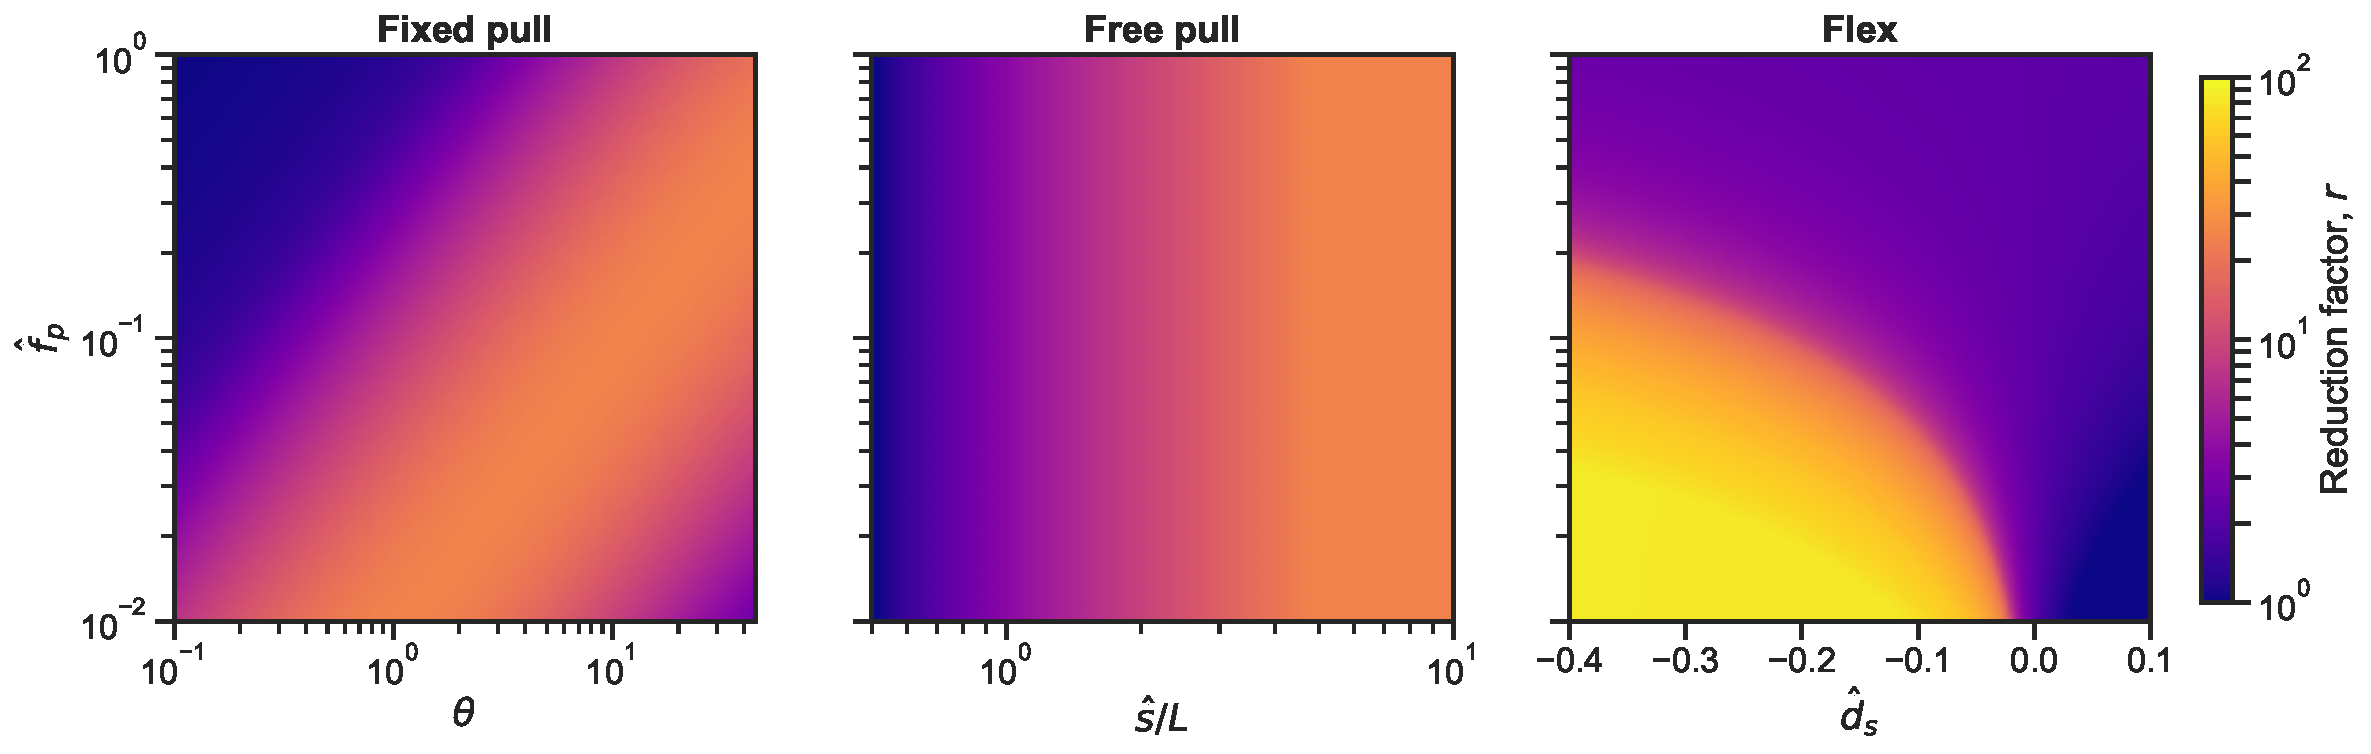
\includegraphics{Reduction_factor-fp}\caption{\textbf{Effect of $\hat{f}_{p}$ on reduction factor.}
Colour plots showing the effect of the dimensionless parameter, $\hat{f}_{p}$,
on the reduction factor for each mode of detachment. Here, we fix
the number of hairs, $N_{t}=25$. \DIFdelbeginFL \DIFdelFL{All values are normalized to }\DIFdelendFL \DIFaddbeginFL \DIFaddFL{The }\DIFaddendFL dimensionless \DIFdelbeginFL \DIFdelFL{forms}\DIFdelendFL \DIFaddbeginFL \DIFaddFL{parameters $\hat{d_{s}}=\frac{d_{s}-l_{h,0}}{w}$ and 
$\hat{s}=\frac{s}{L}$}\DIFaddendFL , as described in text. \label{fig:Reduction-factor_fp}}
\end{figure}

When detachment follows the \emph{fixed pull} method (Figure \ref{fig:Reduction-factor_fp}),
for a constant $\hat{f}_{p}$, the reduction factor increases with
increasing tilt angle, $\theta$, and then decreases, showing a maximum
$r$ of 25 at an intermediate $\theta$. Higher values of $\hat{f}_{p}$
shifts this maximum point to higher values of $\theta$. This trend
relates to the \emph{elastic weakening} effect discussed before. Smaller
values of $\theta$ bring a proportion of hairs under compression,
reducing the adhesion and thus increasing $r$. On further tilting
the array, eventually the proportion of stretched hairs will overcome
the ones under compression, which ultimately reduces $r$ at high
$\theta$. When the individual hairs show strong adhesion (i.e. for
high $\hat{f}_{p}$), a greater tilt is necessary to bring the net
adhesion of the array down.

For the case of detachment via \emph{free pull}, $\hat{f}_{p}$ has
no influence on the reduction factor. On the other hand, shifting
the position of the joint further away from the array (i.e. high
$s/L$) results in large values of $r$. In this scenario, the higher
moment exerted by the array leads to a higher tilt, and thus increases
the reduction factor via \emph{elastic weakening}, saturating to the
maximum value of 25.

For detachment by \emph{flexing}, the reduction factor increases for
higher initial compression of hairs (low $\hat{d}_{s}$). The pad
notably shows a much higher reduction factor at low values of $\hat{f}_{p}$
and $\hat{d}_{s}$, with values as high as 100. Since this mode of
detachment is driven by moment, the pulling force necessary to provide
the moment can be decreased without any limit simply by having a long
lever arm ($\hat{s}_{l}$), i.e., with the joint positioned farther away from the array. 
In contrast, for the previous cases of \emph{free pull} and \emph{fixed pull}, the reduction factor is capped to the maximum number of hairs in the array ($N_{t}=25$). Here, \emph{elastic weakening} can only reduce the array's adhesion force from $N_{t}$
hairs down to a single hair at most.

\paragraph{Effect of $N_{t}$:}

Let us now fix $\hat{f}_{p}=0.1$ and investigate the influence of
the number of hairs, $N_{t}$, on the reduction factor (Figure \ref{fig:Reduction-factor-Nt}).
The colour plots show that high $N_{t}$ increases $r$ irrespective
of the mode of detachment. Under a tilted state, more hairs
are compressed when $N_{t}$ is high, which reduces the net adhesion.
This highlights the advantage of having a split contact design found
in many biological systems. A higher number of hairs offers a better
control over adhesion and thus is more suited for reversible attachment
and detachment during locomotion. The specific trends of reduction
factor for each mode of detachment can be understood by similar arguments
of \emph{elastic weakening}, as discussed in the previous section. 

\begin{figure}[H]
\noindent \begin{centering}
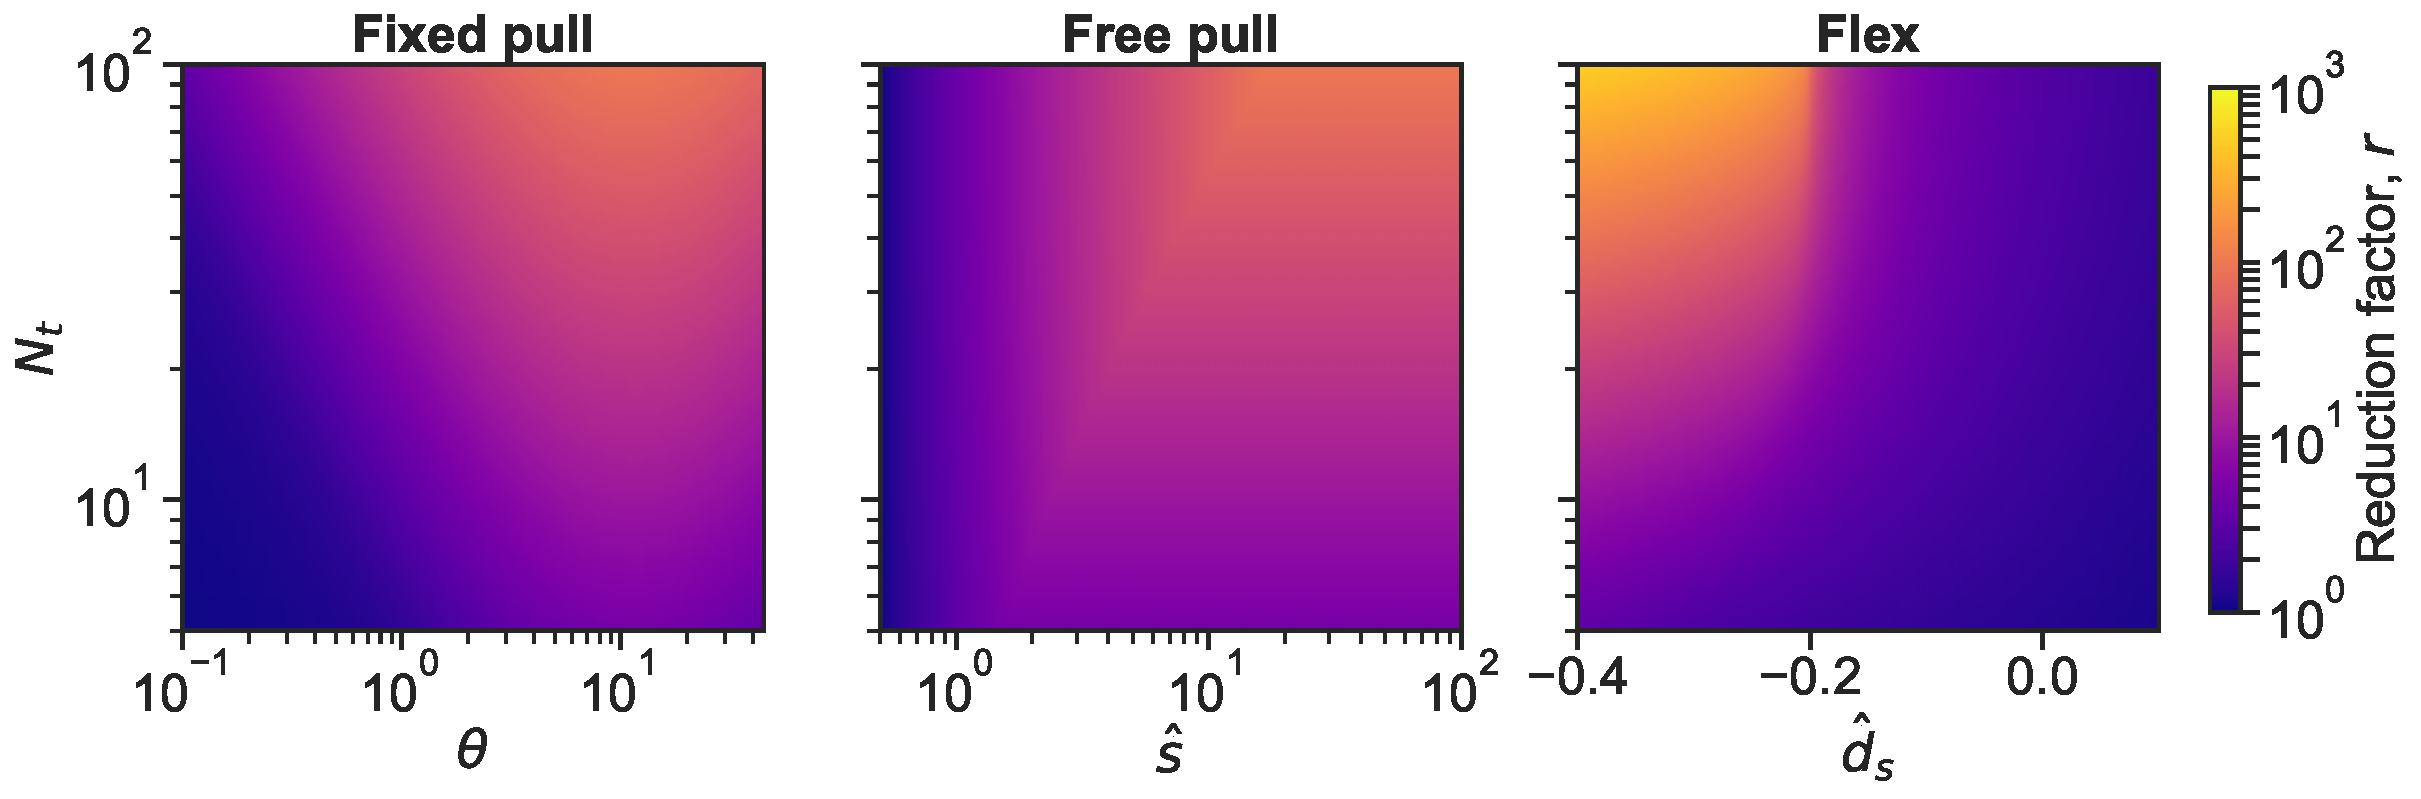
\includegraphics{Reduction_factor-Nt}\caption{\textbf{Effect of $N_{t}$ on reduction factor.} 
Colour plots showing the effect of the number of hairs, $N_{t}$, on
the reduction factor for each mode of detachment. Here, we fix the
dimensionless parameter, $\hat{f}_{p}=0.1$. \DIFdelbeginFL \DIFdelFL{All values are normalized
to }\DIFdelendFL \DIFaddbeginFL \DIFaddFL{The }\DIFaddendFL dimensionless \DIFdelbeginFL \DIFdelFL{forms}\DIFdelendFL \DIFaddbeginFL \DIFaddFL{parameters $\hat{d_{s}}=\frac{d_{s}-l_{h,0}}{w}$ and $\hat{s}=\frac{s}{L}$}\DIFaddendFL , as described in text. \label{fig:Reduction-factor-Nt}}
\par\end{centering}
\end{figure}

\DIFaddbegin \DIFadd{Figures \ref{fig:Reduction-factor_fp} and \ref{fig:Reduction-factor-Nt} can be combined into a single set of colour plots by defining a new dimensionless parameter,  $\chi=\hat{f}_{p} N_{t}=\frac{f_{p}N_{t}}{k_{h}w}$ (see Appendix A). Overall, we see that }\emph{\DIFadd{flex}} \DIFadd{mode of detachment shows the highest reduction factor among the three modes, with the optimal value of $\chi \sim 1$.
}

\DIFaddend \paragraph{Detachment pathways:}

Based on the three modes of detachment discussed in the previous sections,
one can think of several strategies to detach fibrillar adhesive pads
from the surface. To illustrate this, let us consider the adhesive
system of a dock beetle. The beetle is known to have 3 sets of hairy
tarsal adhesive pads in each of their legs, each possessing hairs of different geometries.
To keep our analysis simple, we will assume each leg to have only
two adhesive pads, with identical hairs of mushroom-shaped geometry. The distal
and proximal pads possess roughly 500 and 1000 hairs, respectively \cite{RN19}.
Assuming the pads to be rectangular arrays of $20\times25$ and $40\times25$
hairs, we can model this as a one-dimensional system of 20 and 40
\emph{effective hairs}, respectively, by combining the hairs along the width. Based
on reported measurements \cite{RN79}, the beetle's \emph{effective hair}
is thus considered to have an effective pull-off force, $f_{p}=0.5\times25=12.5$
\textgreek{m}N and effective spring constant, $k_{h}=0.5\times25=12.5$ N m\protect\textsuperscript{-1}.
The beetle's hairs are approximately $l_{h,0}=40$ \textgreek{m}m
long, spaced $w=10$ \textgreek{m}m apart. At end of the tarsal segments, there is 
a claw, around 200 \textgreek{m}m long, and the leg (tibia) is connected roughly
at the end of the proximal tarsal pad. This will put $\hat{s}_{h}=20$ and
$s_{l}/L=1$, measured relative to the right end of the distal pad.
The beetle's leg is assumed to possess two joints which could serve
as a hinge for rotation during detachment (H\textsubscript{1} and H\textsubscript{2}
in Figure \ref{fig:Detachment-pathways} inset). The claw can be used
as an external hinge (H\textsubscript{3}) by flexing the tarsal pad around
it.

Based on the above assumptions, we can come up with force-distance
curves to detach the beetle's leg via various pathways (Figure \ref{fig:Detachment-pathways}).
First, let us assume the joint H\textsubscript{2} to be fixed, such
that both the distal and proximal pads can be combined to behave like a single
long pad with $N_{t}=60$ hairs. Path 1 shows the case where the pad
shows maximum possible adhesion. Here, the combined pad is vertically
pulled upwards while keeping the array perfectly parallel to the surface.
If this combined pad is detached by keeping H\textsubscript{1} fixed and maintaining
a tilt of $1\lyxmathsym{\textdegree}$ with the surface (path 2),
the forces dramatically reduces, with around 10 times reduction in
the adhesion compared to path 1. We can also detach the pad by switching
between the different mechanisms. Path 3 shows one such example, where,
initially the leg is pulled vertically up while keeping H\textsubscript{1}
fixed, stretching the hairs similar to path 1. On reaching point $a$, H\textsubscript{1}
is set free, which results in a sudden drop in force due to the excess
moment by the stretched hairs, tilting the array. Beyond this, the
force curve follows the \emph{free pull} mechanism, with $\thicksim3.5$
times reduction in adhesion. An alternate strategy of switching between
mechanisms would be to first apply a load on the pad (path 4) and
compress the hairs until point $b$. Beyond this point, the claw can
be used as a hinge to detach the pad via flexing it around H\textsubscript{3},
which once again reduces the adhesion force. Now, if we assume the
joint H\textsubscript{2} to be free such that the two pads can behave
distinctly, we can consider the scenario where the proximal pad is
flexed around the distal pad at H\textsubscript{2} while keeping
H\textsubscript{1} fixed (path 5). After the proximal pad has completely
detached, H\textsubscript{1} can be freed up at point $c$ to detach
the distal pad via \emph{free pull} with very little force. This pathway
results in a $\thicksim5$ times reduction in adhesion. 

\begin{figure}[H]
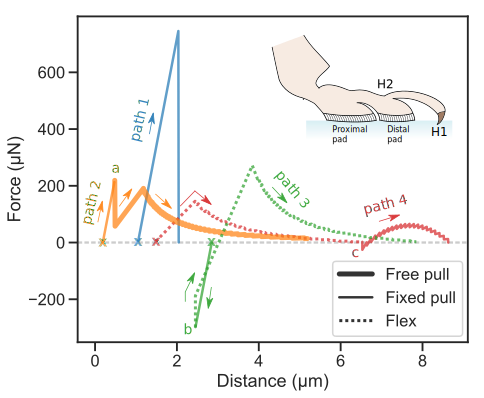
\includegraphics{Detachment_pathways}\caption{\textbf{Beetle leg detachment pathways.}
Force curves showing the theoretical detachment pathways possible for a dock
beetle's leg, as function of distance between the pad and the surface. The curves are
offset laterally for clarity. Colours represent the distinct detachment
pathways, labelled as path 1 to 5, with arrows indicating the
direction of retraction. Points a, b and c indicate instances of switching between the different detachment mechanisms for paths 3, 4 and 5 respectively (see text for details). The different line style denotes the specific
detachment mechanism followed by any region of the pathway. The inset
schematic shows the assumed locations of the different joints or hinges (H\protect\textsubscript{1},
H\protect\textsubscript{2} and H\protect\textsubscript{3}) employed
by the leg. \label{fig:Detachment-pathways}}
\end{figure}

The above analysis illustrates how the design of the beetle's hairy
adhesive pads is suitable for modulating its adhesion. Effective control
and release of its joints can help the insect to reduce the pad's
adhesion, allowing it to detach with little effort. High reduction
in adhesion is seen when the pad is tilted relative to the surface
during detachment, as a result of \emph{elastic weakening}. To the
best of our knowledge, there is no direct experimental evidence that
beetles or any other animal can modulate its adhesion by taking advantage of this effect.
Considering that hair deformation occurs at length scales below 10
\textgreek{m}m, direct observation of this effect on running beetles
would be challenging. A recent study on PDMS micro-pillar arrays,
however, does indeed show a strong reduction in the adhesion force
due to slight misalignments with the surface \cite{RN252}. Based on
previously reported microscopic investigation of freely walking dock
beetles \cite{RN83}, we argue that the following experimental observations
provide support to our proposed model: 1) The detachment was shown
to follow a three-dimensional twist of the leg, which suggests a complex
inhomogeneous deformation of hairs across the array, leading to \emph{elastic
weakening}, which is suited for easy detachment. Similar twisting action during detachment was also observed in flies \cite{niederegger2003} and has been used to easily detach mushroom-shaped artificial adhesive arrays \cite{kang2017}.  2) The beetle can at times instantaneously detach all
its legs and drop itself while upside down. This could be explained
by the beetle freeing up its joints and using just its body weight
to provide the necessary force to detach all its legs via \emph{free
pull} (similar to path 3 above). 3) Only a fraction of the beetle's
pads made contact with the surface during locomotion, which indicates
that the pads should naturally be in a slightly tilted state. This
not only reduces the contact area, but also non-uniformly deforms
the hairs, both leading to a reduction in adhesion for easy detachment.
4) Contact images showed that the array \emph{peels} from the proximal
to distal direction during detachment. However, the beetle's hairs
are attached to a relatively stiff backing \cite{RN53}, so it wouldn't
be able to \emph{peel} its array, since peeling, strictly speaking,
depends on the elastic contribution of a thin flexible backing as
it bends during the process \cite{RN147}. Rather, the \emph{peeling}
observed in the beetle's case should be a result of the pad detaching
from the surface in a tilted orientation, causing the hairs to distinctly detach
in sequence. 5) The time scale of detachment was reported to be an
order of magnitude shorter than the attachment time scale, which could
be a result of the elastic recoil of the leg causing a spontaneous
propagation of the detachment front (Figure \ref{fig:Fixed-pull}). 

There exists a limit to how much the pad can tilt, depending on its
geometry and material properties. Suppose the hair has a maximum linear
elastic strain limit, $\varepsilon_{m}$, and natural length, $l_{h,0}$.
Based on Figure \ref{fig:Schematic}, if the right most hair is compressed
to its elastic limit, one can derive from simple geometry, that, the
corresponding maximum limit in tilt angle is given by: 
\[
\theta_{limit}=\arctan\frac{l_{h,0}\varepsilon_{m}}{\left(N_{t}-1\right)w}
\]
$\theta_{limit}$ will limit the reduction factor for each of the
detachment mechanisms presented. Longer hairs can result in a lateral
collapse or bundling of hairs, imposing an additional constraint on
$\theta_{limit}$. Large deformation of hairs can also lead to buckling,
which will further limit the reduction in adhesion due to the smaller
effective modulus. \DIFdelbegin \DIFdel{Thus, the geometry of the individual hairs is also
crucial in effectively reducing adhesion by }\emph{\DIFdel{elastic weakening}}%DIFAUXCMD
\DIFdel{. 
Ideally, hairswith large diameters would be preferable to eliminate
buckling, and optimally long hairs would provide a large range of angles to which the pad can be tilted while avoiding bundling}\DIFdelend \DIFaddbegin \DIFadd{Buckling could also, interestingly, promote easier detachment in the }\emph{\DIFadd{free pull}} \DIFadd{mode.  
When the compressed hairs at one end of the array buckle, 
there would be an excess clockwise moment in the array system (Figure \ref{fig:Free-pull}). 
This excess moment could subsequently drive the detachment of the remaining hairs.  In the case of biological systems, the ability of an insect to provide the load necessary to tilt and compress its hairy adhesive pad against the surface would further introduce limitations to follow any of the detachment modes discussed here.
All things considered, the geometry and elastic properties of the individual hairs are 
crucial parameters to consider in the design of an optimal array system which shows reversible adhesion via }\emph{\DIFadd{elastic weakening}}\DIFaddend .

Our analysis had been limited to normal forces during detachment. A similar analysis considering the energy required to detach the array will however not yield any \emph{elastic weakening} effect. Since we had assumed a purely elastic system, the initial and final energy of the system would be the same regardless of the mode of detachment, and thus the work of adhesion would remain identical in all scenarios. The reduction of adhesion force is however advantageous since an insect wouldn't then need a strong muscular to system to detach its legs, which are typically capable of attachment forces several times its body weight \cite{ENDLEIN2007}.

\section{Conclusion}

Inhomogeneous deformation of hairs results in significant reductions
in the adhesion of a fibrillar system similar to an insect's tarsal hairy adhesive pads. Such a condition can be achieved
by either 1) pulling the pad while maintaining a constant tilt angle,
2) pulling the pad while maintaining a free tibia-tarsus leg joint or 3) flexing
the pad around the claw. Strategic control of the joint's mobility or claw
can allow the leg to easily switch between the above mechanisms, thus
providing a simple way to reduce adhesion as per necessity. The presence
of a deformable leg can further trigger a spontaneous propagation
of hair detachment due to the leg's elastic recoil, making it suitable
for fast detachment. Arrays with low $\hat{f}_{p}$ and large number
of hairs, with a hair geometry that allows for large deformations
while avoiding buckling and lateral bundling represent the optimal
design conditions to maximize the range of control over adhesion.
The proposed model is supported by previously reported experimental
observations of leg detachment in dock beetles and highlights possible role of the joint and claws to 
enable reversible adhesion. Similar strategies could potentially be adopted in the design of bio-inspired 
artificial fibrillar adhesives to easily switch the adhesion state without the need of asymmetric structures.

\section{Acknowledgment}

We are grateful to Prof. Dr. Hans-J\"{u}rgen Butt and Dr. Thomas Endlein (Max Planck Institute for Polymer Research, Germany) for reviewing the text, and thank Dr. Ren\textcyr{\`\cyre} Hensel
(Leibniz Institute for New Materials, Germany) and
Dr. Bat-El Pinchasik (Tel-Aviv University, Israel) for fruitful discussions. This work was supported by the Deutsche Forschungsgemeinschaft
[Grant number: PI 1351/2-1] and the Max Planck Graduate Center with the Johannes Gutenberg-Universit\"{a}t Mainz [MPGC]. 

\appendix

\section{{\DIFdelbegin \DIFdel{Derivations}\DIFdelend \DIFaddbegin \DIFadd{Reduction factor: master plot}\DIFaddend }}

%DIF < \subsection{Derivations}
\DIFdelbegin %DIFDELCMD < 

%DIFDELCMD < %%%
\DIFdelend \setcounter{figure}{0} \renewcommand{\thefigure}{A.\arabic{figure}} 
\setcounter{equation}{0} \renewcommand{\theequation}{A.\arabic{equation}} 
\DIFaddbegin 

\begin{figure}[H]
\noindent \begin{centering}
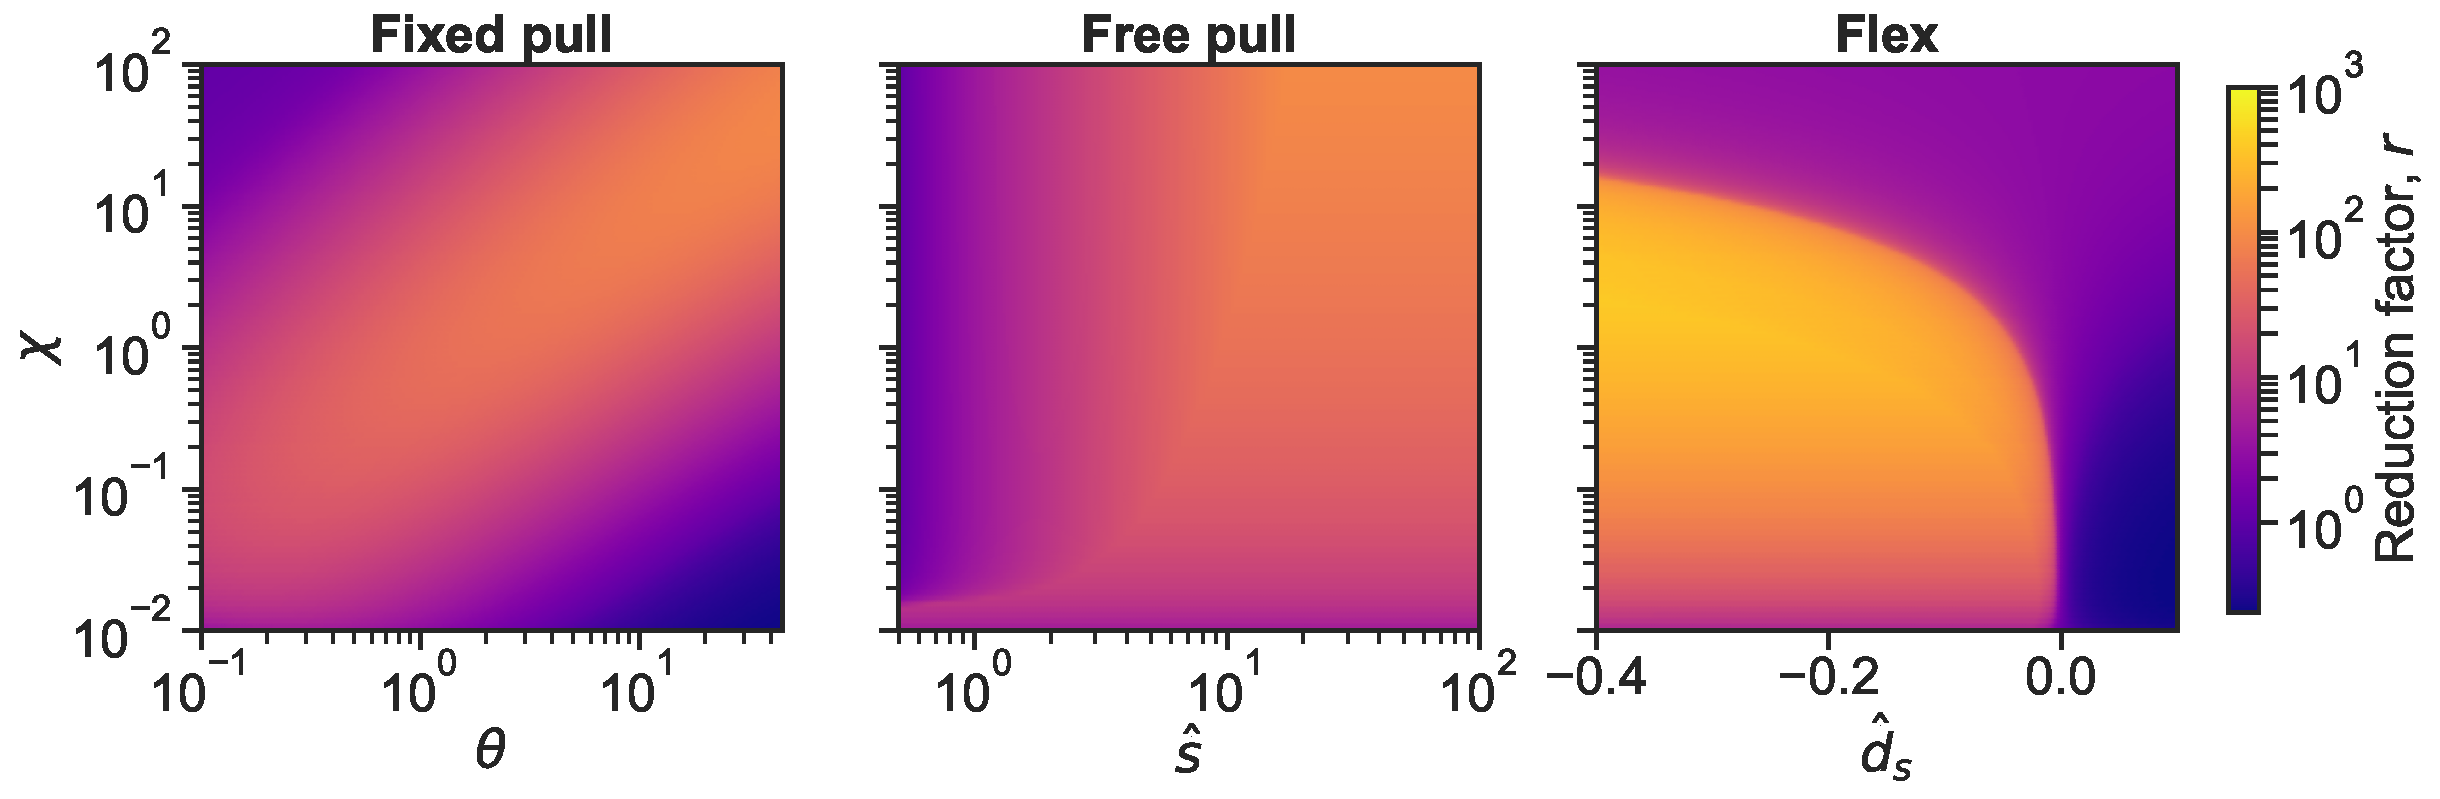
\includegraphics{Reduction_factor-chi}\caption{\textbf{\DIFaddFL{Effect of $\chi$ on reduction factor.}} 
\DIFaddFL{Here, we define a unified dimensionless design parameter $\chi=\frac{f_{p}N_{t}}{k_{h}w}$, combining $\hat{f}_{p}$ and $N_{t}$ into a single number. The dimensionless parameters $\hat{d_{s}}=\frac{d_{s}-l_{h,0}}{w}$ and $\hat{s}=\frac{s}{L}$, as described in text. }\label{fig:Reduction-factor-chi}}
\par\end{centering}
\end{figure}

\section{{\DIFadd{Derivations}}}

%DIF > \subsection{Derivations}
\DIFaddend 

Suppose at a particular instant (Figure \ref{fig:Schematic}), there
are $n$ hairs in contact with the surface. The centre of the region
of the array in contact is at a vertical distance, $d'$, from the
surface. The net force on the whole array is,

\[
F_{net}=\stackrel[i=1]{n}{\sum}k_{h}\left(l_{h,i}-l_{h,0}\right)
\]

$l_{h,i}$ is the length of the $i^{th}$ hair, which is at a horizontal
distance, $x_{i}$, from the centre of the contact region. By simple
geometry, $l_{h,i}=d'-x_{i}\tan\theta$. Substituting $l_{h,i}$ in
above and noting that $\stackrel[i=1]{n}{\sum}x_{i}=0$ by symmetry,
we get:

\[
F_{net}=nk_{h}\left(d'-l_{h,0}\right)
\]

From geometry, $d_{s}$ and $d'$ is related as:

\[
\frac{d_{s}}{\sin\theta}-\frac{d'}{\sin\theta}=s-\frac{\left(n-1\right)w}{2}
\]

Substituting for $d'$, the net force, $F_{net}$, on the pad as a
function of distance, $d_{s}$, is:

\[
F_{net}=nk_{h}\left[d_{s}-l_{h,0}-\left[s-\frac{\left(n-1\right)w}{2}\right]\sin\theta\right]
\]

The above equation is valid for $d_{s}\leq d_{s,max}$ at a particular
value of $n$. We can get $d_{s,max}$ by considering the situation
just before the left most hair is about to detach (Figure \ref{fig:Schematic}).
This hair will be at its maximum length, $l_{h,p}$. Once again from
geometry, we see that $d_{s,max}$ and $l_{h,p}$ is related as:

\[
\frac{l_{h,p}}{\sin\theta}-\frac{d_{s,max}}{\sin\theta}=\left(n-1\right)w-s
\]

Substituting $l_{h,p}=\frac{f_{p}}{k_{h}}+l_{h,0}$ in above and simplifying,
we get:

\[
d_{s,max}=l_{h,0}+\frac{f_{p}}{k_{h}}+\left[s-\left(n-1\right)w\right]\sin\theta
\]

The net moment about the joint due to the deformed hairs of the array
is,

\[
M_{net}=\stackrel[i=1]{n}{\sum}\lambda_{i}k_{h}\left(l_{h,i}-l_{h,0}\right)\cos\theta
\]

Here, $\lambda_{i}=s-\left(\frac{n-1}{2}w-\frac{x_{i}}{\cos\theta}\right)$
is the length of the lever arm between the $i^{th}$ hair and the
joint.

Substituting for $l_{h,i}$ and eliminating $d'$ as before, we get:

\[
M_{net}=\stackrel[i=1]{n}{\sum}k_{h}\cos\theta\left[s-\left(\frac{n-1}{2}w-\frac{x_{i}}{\cos\theta}\right)\right]\left[d_{s}-\left(s-\frac{\left(n-1\right)w}{2}\right)\sin\theta-x_{i}\tan\theta-l_{h,0}\right]
\]

To calculate $\stackrel[i=1]{n}{\sum}x_{i}^{2}$, we follow:

\[
\stackrel[i=1]{n}{\sum}x_{i}^{2}=2\stackrel[i=1]{\frac{n}{2}}{\sum}x_{i}^{2}=2\stackrel[i=1]{\frac{n}{2}}{\sum}\left[w\cos\theta\left(i-\frac{1}{2}\right)^{2}\right]=2w^{2}\cos^{2}\theta\left[\stackrel[i=1]{\frac{n}{2}}{\sum}i^{2}-\stackrel[i=1]{\frac{n}{2}}{\sum}i-\stackrel[i=1]{\frac{n}{2}}{\sum}\frac{1}{4}\right]
\]

Using the identities $\stackrel[i=1]{N}{\sum}i^{2}=\frac{N\left(N+1\right)}{2}$
and $\stackrel[i=1]{N}{\sum}i^{2}=\frac{N\left(N+1\right)\left(2N+1\right)}{6}$
and simplifying, we get $\stackrel[i=1]{n}{\sum}x_{i}^{2}=n\left(\frac{n^{2}-1}{12}\right)w^{2}\cos^{2}\theta$.
This, together with $\stackrel[i=1]{n}{\sum}x_{i}=0$ (by symmetry),
the expression for $M_{net}$ above can be simplified to finally get:

\[
M_{net}=nk_{h}\cos\theta\left[\left(d_{s}-l_{h,0}\right)\left[s-\frac{\left(n-1\right)w}{2}\right]-\left\{ \left[s-\frac{\left(n-1\right)w}{2}\right]^{2}+\frac{n^{2}-1}{12}w^{2}\right\} \sin\theta\right]
\]

\bibliography{references}

\end{document}
